\documentclass{TDP003mall}

\usepackage{listings}
\usepackage{graphicx}
\usepackage{float}
\usepackage{verbatim}

\usepackage{hyperref}
\hypersetup{
  colorlinks=true,
  linkcolor=black,
  filecolor=blue,
  urlcolor=blue,
}

\newcommand{\version}{Version 1.0}
\author{Jimmie Roos, \url{jimro697@student.liu.se}\\
        Sebastian Grunditz, \url{sebgr273@student.liu.se}}
\title{Installationsmanual för Portföljsystem}
\date{2018-09-20}
\rhead{Jimmie Roos\\
      Sebastian Grunditz}



\begin{document}
\projectpage
\tableofcontents
\clearpage
\section{Revisionshistorik}
\begin{table}[!h]
\begin{tabularx}{\linewidth}{|l|X|l|}
\hline
Ver. & Revisionsbeskrivning & Datum \\\hline
1.0 & Dokument skapat & 20/9\\\hline
\end{tabularx}
\end{table}

\section{Grundläggande information för installation}
Allt kommer att installeras med hjälp av terminalen i Linux. Den öppnas med:
\begin{lstlisting}[language=bash]
  CTRL-ALT-t
\end{lstlisting}
För att följa manualen behöver man ha antingen Linux Mint eller Ubuntu installerat.
\subsection{Programversioner}
Nedan är en lista med versionerna på de program som finns med i den här manualen.
\begin{itemize}
  \item python 3.6
  \item Jinja 2.0
  \item Flask 1.0.2
  \item Ubuntu 18.04
  \item Atom 1.30.0
  \item git 2.17.1
  \item HTML5
  \item CSS3
\end{itemize}


\section{Python3}
\subsection{Installation av Python3}
Prova skriv in python3 i terminalen och klicka på ENTER för
att se om det är installerat. Om det ser ut som bilden så är det installerat.
\begin{figure}[H]
  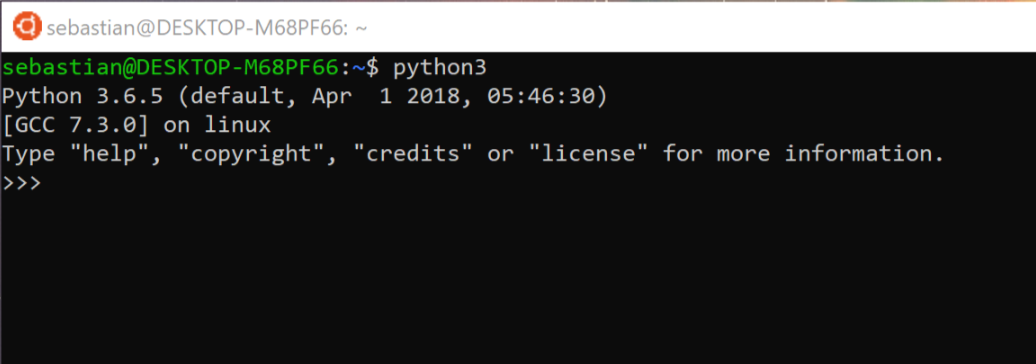
\includegraphics[width=0.6\linewidth]{python.png}
  \caption{En vild pythonterminal}
  \label{fig:python}
\end{figure}

Annars så måste vi installera det. Det gör vi genom att skriva:
\begin{lstlisting}[language=bash]
  $ sudo apt install python3
\end{lstlisting}

\subsection{Installation av pip och virtualenv}
Installation av pip är lite krångligare än python3, men inte jättesvår.
Man får även med python3 vrtualenv när man installerar.
\begin{lstlisting}[language=bash]
  $ sudo apt-get install python3-pip python3-dev build-essential python3-venv

  $ sudo pip install --upgrade pip

  $ sudo pip install --upgrade virtualenv
\end{lstlisting}

\subsection{Köra en python3 fil}
För att köra en python3 fil i terminalen behöver man ha:
\begin{lstlisting}[language=bash]
  #! /usr/bin/env python3
\end{lstlisting}

i toppen på .py filen. Första gången man ska köra den kommer det se ut
ungefär som:
\begin{lstlisting}[language=bash]
  $ chmod u+x <filnamn>.py

  $ python3 ./<filnamn>.py
\end{lstlisting}
``chmod'' kommandot behöver man bara köra en gång per fil, då den gör så att man
får rättigheter att köra den.

\section{Atom}
\subsection{Installation}
En editor som är lätt att använda är atom. Den installerar vi genom att skriva
dessa kommandon:
\begin{lstlisting}[language=bash]
  $ curl -sL https://packagecloud.io/AtomEditor/atom/gpgkey | sudo apt-key add -

  $ sudo sh -C echo 'deb [arch=amd64] https://packagecloud.io/AtomEditor/atom/any
    any main}' > /etc/apt/sources.list.d/atom.list

  $ sudo apt-get update

  $ sudo apt-get install atom
\end{lstlisting}


\section{Git}
\subsection{Installation}
De flesta linuxinstallationer kommer med git installerat men det kan vara bra att
kolla så det är uppdaterat eller om det saknas. Skriv in dessa kommandon i ordning
och följ instruktionerna på skärmen.

\begin{lstlisting}[language=bash]
  $ sudo apt-get update

  $ sudo apt-get upgrade

  $ sudo apt-get install git
\end{lstlisting}

\subsection{Komma igång}
När man installerat git, vill man få igång ett repository, en mapp som länkas mot github
eller gitlab, beroende på vad du använder. Först behöver man en ssh-nyckel, som används
för att identifiera datorn. Den skapar man med:
\begin{lstlisting}[language=bash]
  $ ssh-keygen -t rsa -C <Valfritt namn> -b 4096
\end{lstlisting}
De prompter som kommer upp kan man bara trycka förbi med ENTER. När den är skapad
ska man kopiera publika nyckeln, och lägga till i SSH-nyckel kategorien på hemsidan.
Detta kan man göra genom att öppna id\_rsa.pub med hjälp av till exempel Atom. Kopiera
allt med CTRL+A och CTRL+C.\\
Om du har skapat ett eget repository på motsvarande
hemsida, står det hur man gör för att komma igång med Git lokalt. Om du har tillgång
till ett repository som redan har filer i sig ska du göra följande:
\begin{lstlisting}[language=bash]
  $ cd <mapp>

  $ git init

  $ git remote add origin <git-url>

  $ git pull origin master
\end{lstlisting}

\section{Flask och Jinja2}
\subsection{Installation}
Det sista vi behöver är Flask och Jinja2 för att kunna göra en hemsida med både
databas, och snygg framsida. Vi behöver även skapa en virtuell miljö, med hjälp
av virtualenv som vi installerade tillsammans med PIP. Det gör man genom att skriva:
\begin{lstlisting}[language=bash]
  $ mkdir <projektnamn>

  $ cd <projectnamn>

  $ python3 -m venv venv

  $ . venv/bin/activate

  $ sudo pip3 install flask
\end{lstlisting}
Vi använder . venv/bin/activate kommandot för att komma in i vår virtualenv.
För att komma ut ur virtualenv så skriver vi deactivate.
Jinja2 är en del av flask och installeras tillsammans med flaskinstallationen.

\subsection{Användning}
För att göra en fil körbar i Flask så gå vi till mappen där filen finns och skriver:
\begin{lstlisting}[language=bash]
  $ export FLASK_APP=<filnamn>.py

  $ flask run
\end{lstlisting}
Där <filnamn> är huvudfilen i projektet.

\section{Felsökning och underhåll}
\subsection{Felsökning Flask}
Flask sparar ingen log per automatik, utan skriver ut felmeddelanden i den terminal
appen körs i. För att spara loggen, kan man till exempel skriva till `` > log.txt''
till sitt run kommando, så det ser ut som exemplet:
\begin{lstlisting}[language=bash]
  $ flask run > log.txt
\end{lstlisting}
Om du bara får
\begin{lstlisting}[language=bash]
  * Running on http://127.0.0.1:5000/ (Press CTRL+C to quit)
\end{lstlisting}
så har du gjort rätt, och all annan info som Flask skickar när den kör, kommer hamna i
``log.txt''
För mer information om felhantering i
Flask kan man gå in på \href{http://flask.pocoo.org/docs/1.0/errorhandling/#application-errors}{Flask Logging}.

\subsection{Underhåll}
För att se till att allt är uppdaterat kan vi använda oss av kommadot:
\begin{lstlisting}
  $ sudo apt-get update

  $ sudo apt-get upgrade
\end{lstlisting}

\subsubsection{Git}
Gör det som vana att alltid göra en ``pull'' innan man ska börja koda. Detta gör man
med:
\begin{lstlisting}[language=bash]
  $ git pull
\end{lstlisting}
Detta gör att man inte får några konflikter med den ``branchen'' man arbetar i just nu.
När man är färdigkodad, så behöver man ``pusha'' det man gjort. Detta gör man med:
\begin{lstlisting}[language=bash]
  $ git add .

  $ git commit -m '<Ett beskrivande meddelande om dagens arbete>'

  $ git push
\end{lstlisting}
Mer info om ``branches'' och annat om Git hittar du \href{https://help.github.com/}{här}.
\subsection{Projektmodifiering}
Det finns i samma mapp som alla html-filer och så, en .json-fil, som agerar databas.
\subsubsection{Lägga till projekt}
För att lägga till ett färdigt projekt, börja med att kopiera html-mallen som finns
och döp om den till <projektnamn>.html med:
\begin{lstlisting}[language=bash]
  $ cp mall.html <projektnamn>.html
\end{lstlisting}
Sedan öppnar man databasen i Atom för att lägga till all information. Titta på
hur strukturen är på de tidigare projekten, kopiera ett av dem, och byt ut
informationen mot det som ska beskriva det projekt du vill lägga till.

\subsubsection{modifiera ett existerande projekt}
För att modifiera ett existerande projekt, öppna databasen i Atom. Leta sedan rätt
på det projekt du vill modifiera och ändra på den aktuella datan.


\end{document}
